\documentclass[10pt]{article}
\usepackage{icmlko}

\icmlmeta{IP 파운데이션 월드모델}{242}{겹말이라고 다 뺄 수 있는 것은 아니다}{$\rho \geq 0.95$ 는 선형의 눈이다 --- 셋이 겹치는데 빼도 되는 것은 하나뿐이었다}

\begin{document}

\twocolumn[
\icmlheader

\begin{abstract}
노트 240이 붙인 가드 열일곱 \textbf{겹말}이 지금 판에서 겹치는 축 쌍
\textbf{열다섯}을 찾았고, 전부 같은 모양이었다 --- 검색 · 위키 시계열의
\texttt{level} · \texttt{volatility} · \texttt{peak\_ratio} 가 \textbf{한
방향을 세 번} 싣고 있다(만화 \texttt{wiki\_volatility} $\sim$
\texttt{wiki\_peak\_ratio} 는 $\rho{=}1.000$). 세 겹을 한 겹으로 줄이면 판이
어떻게 되나. 하나씩 빼서 쟀다. \textbf{셋이 서로 $\rho \geq 0.95$ 인데 정보는
전혀 다르다.} \texttt{peak\_ratio} 둘을 빼면 \textbf{세 정식화가 다 올라간다}
(F21 $+$0.0007 · F18 $+$0.0011 · F23 $+$0.0021) --- 축이 둘 줄고 판이 오른다.
\texttt{volatility} 를 마저 빼면 \textbf{나무가 무너지고}(F18 $-$0.0054,
$t{=}-2.11$) F23도 $-$0.0023 이다. \texttt{level} 을 빼면 F18 $-$0.0099
($t{=}-3.33$) · F23 $-$0.0062($t{=}-2.30$)로 제일 크게 내린다. 정보의 크기는
\textbf{level $\gg$ volatility $>$ peak\_ratio $\approx$ 0} 이다. 교훈은
가드 자체에 관한 것이다 --- \textbf{$\rho \geq 0.95$ 는 선형의 눈이라 후보를
짚을 뿐이고, 나무는 남은 5\%를 쓴다.} 겹말은 여전히 이름표이지 거부권이
아니다. \texttt{peak\_ratio} 둘만 뺐다. 판 \textbf{0.4548 $\to$ 0.4569},
축 19 $\to$ 17, 겹말 15쌍 $\to$ 3쌍.
\end{abstract}
]

\section{한 방향을 세 번 싣고 있었다}

노트 240은 새 축이 기존 축의 다시 쓰기인지 보는 가드를 붙이면서, 정작
\emph{지금 판}에 그런 쌍이 열다섯 개 있다는 것을 부수적으로 발견했다. 목록이
한눈에 읽힌다.

\begin{center}\small
\begin{tabular}{lrl}
\hline
도메인 & $\rho$ & 쌍 \\
\hline
만화 & $+$1.000 & \texttt{wiki\_volatility} $\sim$ \texttt{wiki\_peak\_ratio} \\
펀딩 & $+$0.999 & \texttt{trend\_volatility} $\sim$ \texttt{trend\_peak\_ratio} \\
웹툰 & $+$0.998 & \texttt{wiki\_volatility} $\sim$ \texttt{wiki\_peak\_ratio} \\
펀딩 & $+$0.998 & \texttt{trend\_level} $\sim$ \texttt{trend\_volatility} \\
만화 & $+$0.997 & \texttt{wiki\_level} $\sim$ \texttt{wiki\_peak\_ratio} \\
\multicolumn{3}{c}{\dots\ 열 쌍 더, 전부 같은 세 축} \\
\hline
\end{tabular}
\end{center}

시계열에서 뽑는 네 축 중 셋이다 --- 수준 · 변동성 · 봉우리 비. 남은 하나는
\texttt{momentum} 인데 겹치지 않는다. 그러면 세 겹을 한 겹으로 줄여도
되는가.

\section{셋을 하나씩 뺐다}

\begin{figure}[t]
\centering
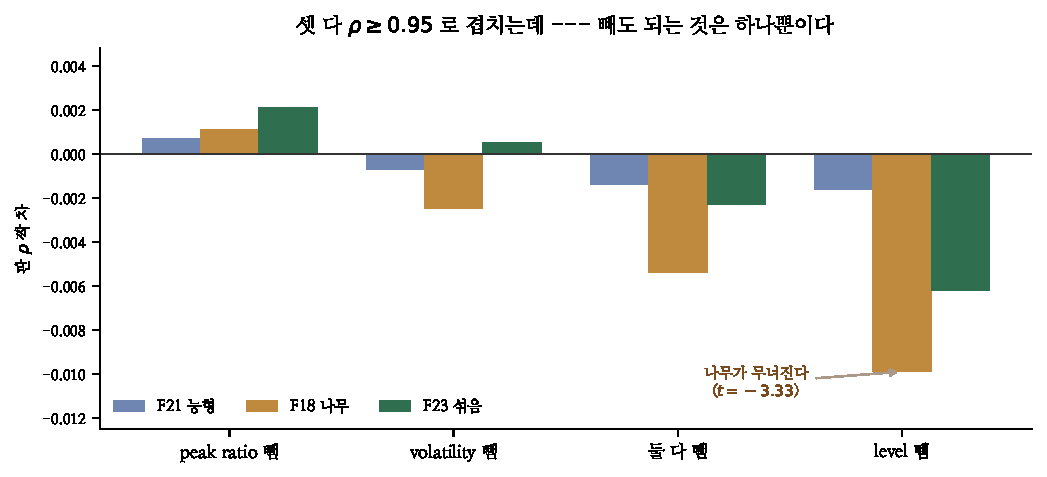
\includegraphics[width=\columnwidth]{figs/drops.pdf}
\caption{무엇을 빼면 무엇이 무너지나. 셋 다 서로 $\rho \geq 0.95$ 인데
결과가 정반대다.}
\end{figure}

\begin{center}\small
\begin{tabular}{lrrr}
\hline
뺀 것 & F21 능형 & F18 나무 & F23 판 \\
\hline
\texttt{peak\_ratio} 둘 & $+$0.0007 & $+$0.0011 & $\mathbf{+0.0021}$ \\
\texttt{volatility} 둘 & $-$0.0007 & $-$0.0025 & $+$0.0005 \\
둘 다 (넷) & $-$0.0014 & $-$0.0054 & $-$0.0023 \\
\texttt{level} 둘 & $-$0.0016 & $-$0.0099 & $-$0.0062 \\
\hline
\end{tabular}
\end{center}

\texttt{peak\_ratio} 는 \textbf{세 정식화가 다 올라간다}. 축이 둘 줄고 판이
오르는 것은 순수한 이득이다. \texttt{volatility} 는 F23만 보면 $+$0.0005 로
동점 같지만 F21 $-$0.0007($t{=}-1.83$) · F18 $-$0.0025 로 두 부품이 다
내려간다. 둘을 같이 빼면 \textbf{나무가 무너진다}(F18 $-$0.0054,
$t{=}-2.11$). \texttt{level} 은 제일 크게 내린다(F18 $-$0.0099,
$t{=}-3.33$).

\section{$\rho \geq 0.95$ 는 선형의 눈이다}

$\rho{=}1.000$ 인 쌍이 있는데 왜 한쪽만 뺄 수 있나. 순위 상관은 단조
관계를 재고, \textbf{능형은 단조 관계 이상을 못 본다} --- 두 열이 단조로
같으면 능형에게는 정말로 같은 열이다. 그런데 \textbf{나무는 문턱에서
자른다.} $\rho{=}0.96$ 은 ``거의 같다''이지 ``같다''가 아니고, 어긋나는
4\%가 하필 문턱 근처에 있으면 나무는 그것으로 가른다.

그래서 노트 240이 ``겹말은 거부권이 아니라 이름표''라고 적어 둔 것이
이번에 값을 했다. 가드가 열다섯 쌍을 짚어 줬고, \textbf{그중 실제로 뺄 수
있는 것은 여섯 쌍(= peak\_ratio 관련) 뿐}이었다. 가드가 거부권이었다면 판을
$-$0.0023 내렸을 것이다.

\begin{figure}[t]
\centering
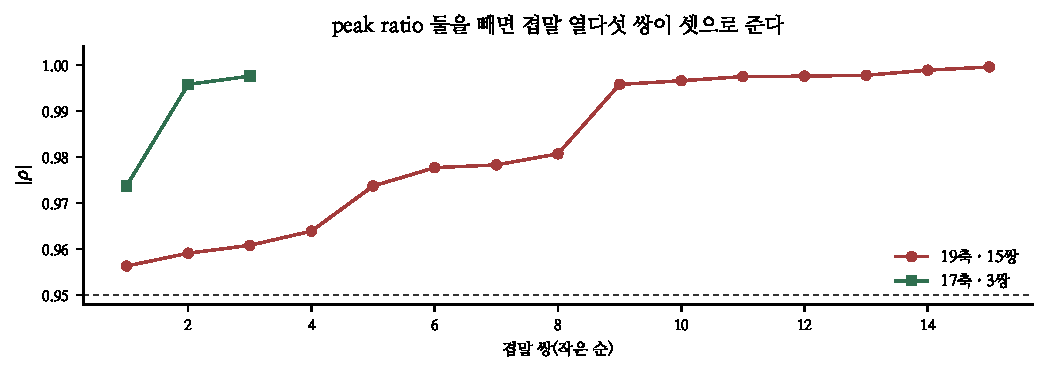
\includegraphics[width=\columnwidth]{figs/pairs.pdf}
\caption{\texttt{peak\_ratio} 둘을 빼면 겹말 열다섯 쌍이 셋으로 준다.
남은 셋은 \texttt{level} $\sim$ \texttt{volatility} 인데, 위 표가 그 둘은
못 뺀다고 말한다.}
\end{figure}

\section{둘만 뺀다}

\texttt{trend\_peak\_ratio} 와 \texttt{wiki\_peak\_ratio} 를 뺐다.

\begin{center}\small
\begin{tabular}{lrrr}
\hline
 & 축 & F23 판 & 겹말 쌍 \\
\hline
전 & 19 & 0.4548 & 15 \\
후 & \textbf{17} & \textbf{0.4569} & \textbf{3} \\
\hline
\end{tabular}
\end{center}

근거는 \textbf{겹말 구조}다 --- 라벨을 안 보는 학습 구간 순위 상관이 후보를
짚었고, 유보 수는 확인이다. 축을 빼는 것도 더하는 것과 같은 설계 선택이라
유보로 정하면 안 된다는 노트 239의 규칙을 그대로 지켰다.

노트 240이 판을 0.4584에서 0.4546으로 되돌렸고(취소), 이번에 0.4569로
올라왔다. \textbf{되돌린 값보다 낮고, 이번 것은 새 자료가 아니라 뺀 것으로
얻었다.}

\paragraph{남은 것}
\begin{center}\small
\begin{tabular}{ll}
\hline
갈래 & 왜 \\
\hline
남은 겹말 3쌍 & \texttt{level}$\sim$\texttt{volatility} --- 못 뺀다. 합치면? \\
안쪽 신호 부호 & 노트 241에서 반대로 나왔다. 세 조각이 짧은가 \\
$\tau$ 칼날 & 잡음 열 하나로 꺼진다(6 중 3) \\
\texttt{momentum} & 겹치지 않는 유일한 시계열 축. 혼자 얼마나 하나 \\
\hline
\end{tabular}
\end{center}

\paragraph{규약} 겹말 가드가 짚은 쌍은 \textbf{빼 보고 정한다.} 능형과
나무를 따로 본다 --- F23만 보면 \texttt{volatility} 는 동점으로 보이는데
부품 둘이 다 내려가고 있다.

\end{document}
